\documentclass[12pt, a4paper]{article}
\usepackage[utf8]{inputenc}
\usepackage[english]{babel}
\usepackage{amsmath}
\usepackage{amssymb}
\usepackage{amsfonts}
\usepackage{csquotes}
\usepackage{mathtools}
\usepackage{graphicx}
\usepackage{geometry}
\usepackage{setspace}
\usepackage{longtable}
\usepackage{float}
\usepackage{comment}
\usepackage[colorlinks=true, allcolors=blue]{hyperref}

\usepackage[style=authoryear]{biblatex}
\addbibresource{Bibliography.bib}

\geometry{top = 2.5cm, bottom = 2.5cm, left= 3cm, right= 3cm}

\title{Properties of a Vibrating String}
\author{Lee Farrugia \\ Experiment 13 \\ Group 1A}

\date{$22^{\text{nd}}$ November 2021}

\begin{document}

\maketitle

\section*{Aim}
The aim of this experiment is to obtain the frequency of the tuning fork using the principle of resonance.

\section*{Diagram}
\begin{figure}[H]
    \centering
    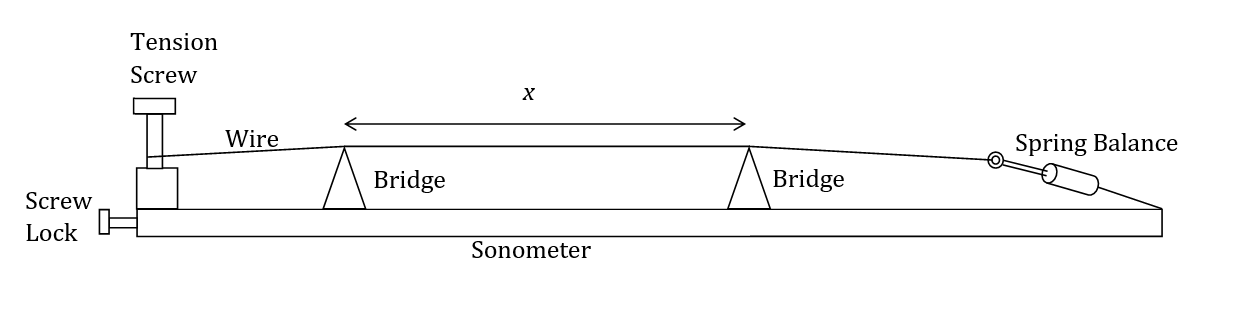
\includegraphics[scale=0.4]{Diagram.png}
    \caption{Apparatus setup}
    \label{fig:setup}
\end{figure}

\section*{List of Apparatus}
Wire, spring balance, sonometer, tuning fork, paper riders, two bridges, micrometer screw gauge, rubber pad.

\section*{Language and Packages}
Python 3.9.7, Numpy, Matplotlib.pyplot, smypy, math, Pandas. 

\section*{Procedure}
\begin{enumerate}
    \item The diameter of the wire was measured using the micrometer screw gauge, at three different positions, twice at each position at right angles to each other.
    \item The apparatus was set up as shown in the diagram above.
    \item The tension screw was tightened so that the wire was under a tension $T$ of 10 N.
    \item A small paper rider was placed on the wire.
    \item The tuning fork was set by hitting it against the rubber pad.
    \item The vibrating tuning fork was then placed on one of the bridges, while the other was moved slowly until the paper rider fell off. At this point resonance was achieved.
    \item The distance $x$ between both bridges was measured using the meter ruler.
    \item The whole procedure was repeated again, each time the tension increased by 5 N until five sets of readings were obtained. This was done until five repeated readings at each tension value were obtained.
\end{enumerate}

\section*{Precautions}
\begin{itemize}
    \item[-] Small distances of $x$ were used so that the resonance that occurred was in the first harmonic.
    \item[-] Tension was first increased to the maximum and then decreased to the minimum when taking the readings.
    \item[-] The micrometer screw gauge was tightened using the ratchet so as not to over tighten it.
    \item[-] When taking readings the micrometer screw gauge was locked. 
    \item[-] The different points at which the thickness was measured were far apart from each other.
\end{itemize}

\section*{Sources of Error}
\begin{itemize}
    \item[-] The repeated usage of the string by different students will have stretched out the string thus distorting the diameter and resonance distance.
    \item[-] As the force of the hit applied to the tuning fork may have not been constant a different amplitude of resonance might have been achieved thus making the paper rider fall off easier.
    \item[-] The wire might not have been perfectly uniform.
    \item[-] The wire might have had some impurities. 
    \item[-] The scale error of the micrometer screw gauge.
\end{itemize}

\section*{Data and Graphs}
\begin{longtable}{| c | c | c | c |}
\caption{Diameter and Radius Readings}
\label{tab:diamater table}\\
\hline d/mm  & d/m & r/m\\
\hline \textpm 0.01 & \textpm 1$\times 10^{-5}$ & \textpm 1$\times 10^{-5}$\\ \hline
\endfirsthead

\hline d/mm  & d/m & r/m\\
\hline \textpm 0.01 & \textpm 1$\times 10^{-5}$ & \textpm 1$\times 10^{-5}$\\ \hline
\endhead

0.36  & 0.00036 & 0.000180\\\hline
0.36  & 0.00036 & 0.000180\\\hline
0.37  & 0.00037 & 0.000185\\\hline
0.36  & 0.00036 & 0.000180\\\hline
0.36  & 0.00036 & 0.000180\\\hline
0.36  & 0.00036 & 0.000180\\\hline
\end{longtable}

\begin{longtable}{| c | c | c | c | c | c | c | c | c | c|}
\caption{Distance and Force Readings}
\label{tab:distances table}\\
\hline $\text{F}_1/\text{N}$ & $\text{x}_1/\text{m}$ & $\text{F}_2/\text{N}$ & $\text{x}_2/\text{m}$ & $\text{F}_3/\text{N}$ & $\text{x}_3/\text{m}$ & $\text{F}_4/\text{N}$ & $\text{x}_4/\text{m}$ & $\text{F}_5/\text{N}$ & $\text{x}_5/\text{m}$ \\

\hline \textpm 1 & \textpm 1$\times 10^{-3}$ & \textpm 1 & \textpm 1$\times 10^{-3}$ & \textpm 1 & \textpm 1$\times 10^{-3}$ & \textpm 1 & \textpm 1$\times 10^{-3}$ & \textpm 1 & \textpm 1$\times 10^{-3}$ \\ \hline
\endfirsthead

\hline $\text{F}_1/\text{N}$ & $\text{x}_1/\text{m}$ & $\text{F}_2/\text{N}$ & $\text{x}_2/\text{m}$ & $\text{F}_3/\text{N}$ & $\text{x}_3/\text{m}$ & $\text{F}_4/\text{N}$ & $\text{x}_4/\text{m}$ & $\text{F}_5/\text{N}$ & $\text{x}_5/\text{m}$ \\

\hline \textpm 1 & \textpm 1$\times 10^{-3}$ & \textpm 1 & \textpm 1$\times 10^{-3}$ & \textpm 1 & \textpm 1$\times 10^{-3}$ & \textpm 1 & \textpm 1$\times 10^{-3}$ & \textpm 1 & \textpm 1$\times 10^{-3}$ \\ \hline
\endhead

10 & 0.119 & 15 & 0.139 & 20 & 0.155 & 25 & 0.168 & 30 & 0.185 \\ \hline
10 & 0.120 & 15 & 0.138 & 20 & 0.156 & 25 & 0.170 & 30 & 0.185 \\ \hline
10 & 0.118 & 15 & 0.139 & 20 & 0.155 & 25 & 0.169 & 30 & 0.183 \\ \hline
10 & 0.120 & 15 & 0.139 & 20 & 0.154 & 25 & 0.171 & 30 & 0.184 \\ \hline
10 & 0.120 & 15 & 0.139 & 20 & 0.153 & 25 & 0.170 & 30 & 0.184 \\ \hline    
\end{longtable}

\begin{figure}
    \centering
    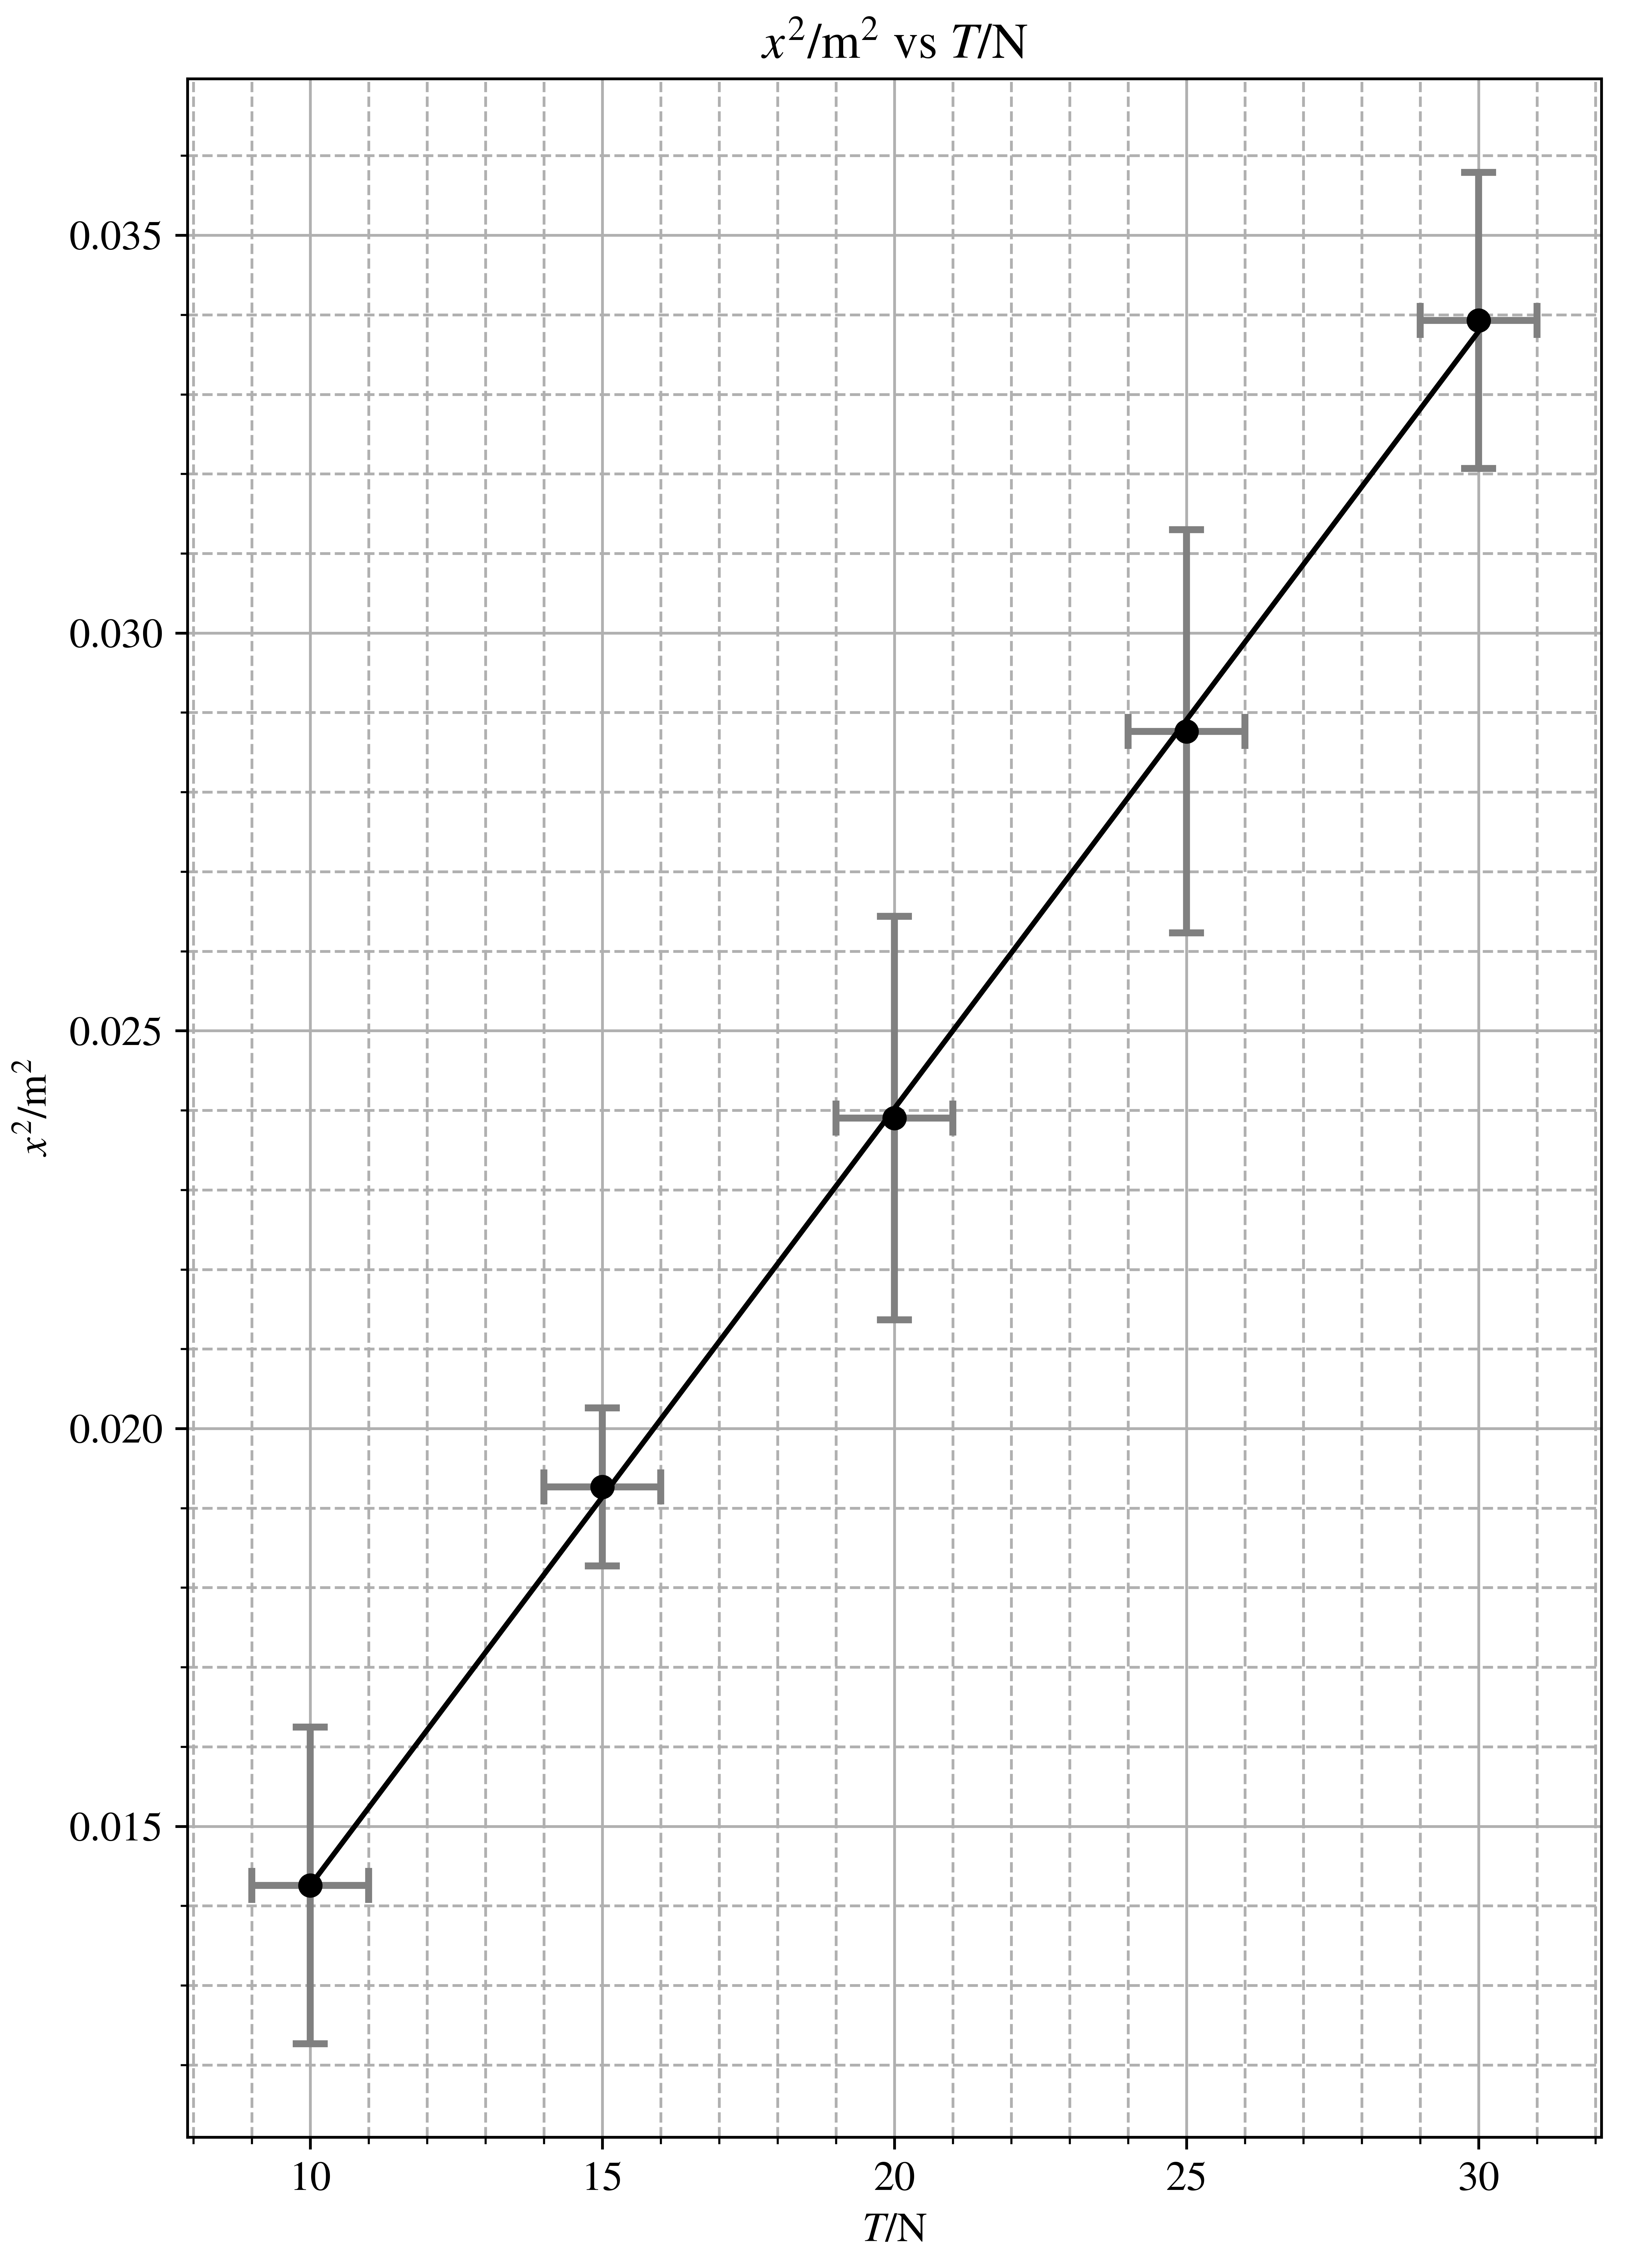
\includegraphics[scale=0.9]{x2vsTgraph.png}
    \caption{Graph of Distance vs Tension}
    \label{fig:x2graph}
\end{figure}

\section*{Calculations}
The data collected during the experiment was inputted into an excel sheet, which was then read by the program using the following line of code:
\begin{verbatim}
    data = pd.read_excel(`Experiment 13.xlsx').
\end{verbatim}
The averages of the readings obtained were found using the following lines of code:
\begin{verbatim}
    r = data[`r/m'].mean()
    x = data[`x1/m'].mean(), data[`x2/m'].mean(),
        data[`x3/m'].mean(), data[`x4/m'].mean(),
        data[`x5/m'].mean()
    T = data[`f1/N'].mean(), data[`f2/N'].mean(),
        data[`f3/N'].mean(), data[`f4/N'].mean(), 
        data[`f5/N'].mean().
\end{verbatim}
The equation given that links the distance between bridges $x$ and the tension $T$ of the wire is:
\begin{equation} \label{eq: distance tension}
    x = \sqrt{\frac{T}{4 \pi \rho r^2 f^2}}\,,
\end{equation}
where $x$ is the distance between the bridges, $T$ is the tension of the wire, $\rho$ is the density of the wire, and $f$ is the frequency of the tuning fork. In order to plot, it was rearranged to:
\begin{equation}
    x^2 = \frac{T}{4 \pi \rho r^2 f^2}\,.
\end{equation}
When this equation is compared to the straight line equation $y = m x + c$ it is noted that the gradient $m$ corresponds to $\frac{1}{4 \pi \rho r^2}$ and thus the following lines of code were used in order to obtain the gradient and the line of best fit for the data:
\begin{verbatim}
    coeffs, cov = np.polyfit(T, x2, 1, cov=True)
    poly_function = np.poly1d(coeffs)
    trendline = poly_function(T)
    m = coeffs[0],
\end{verbatim}
where the error of the gradient was found by square rooting the correct position of the co-variance matrix. This was done using the following line of code:
\begin{verbatim}
    deltam = np.sqrt(cov[0][0]).
\end{verbatim}
In order to obtain the frequency of the tuning fork, the gradient $\frac{1}{4 \pi \rho r^2 m}$ was used which resulted to be 544.57 Hz. This was done through the following line of code:
\begin{verbatim}
    freq = np.sqrt(1/ (constant * r**2  * coeffs[0])),
\end{verbatim}
where the constant refers to $\frac{1}{4 \pi \rho}$, coeffs[0] is the gradient obtained from before. Next the error for $r$ was obtained using the following line of code:
\begin{verbatim}
    deltar = 2.57 * (np.std(data[`r/m'])/np.sqrt(6)).
\end{verbatim}
Next the combined error for the frequency was obtained using the following equation:
\begin{align} \label{eq: Combined error eq}
    \Delta f &= \sqrt{\left(\frac{\partial f}{\partial r}\Delta r \right)^2 + \left(\frac{\partial f}{\partial m} \Delta m \right)^2}\,,\\
    \nonumber \Delta f &=\sqrt{\left(\frac{(\pi \rho m)^{\frac{1}{2}}}{2\pi \rho r^2 m} \Delta r \right)^2 +\left(\frac{(\pi \rho m)^{\frac{1}{2}}}{4\pi \rho r m^2} \Delta m \right)^2}\,,\\
    \nonumber \Delta f &= \pm 6.48\text{Hz}\,.
\end{align}
This was achieved using the following lines of code:
\begin{verbatim}
    def freqerr(d, e, f, deltar, deltam):
        a = Symbol(`a')
        b = Symbol(`b')
        c = Symbol(`c')
        equation = (1/(c * (a**2) * b))**0.5
        diff_a = Derivative(equation, a)
        diff_b = Derivative(equation, b)
        da = diff_a.doit()
        db = diff_b.doit()
        dr = da.subs({a : d, b : e, c : f}).evalf()
        dm = db.subs({a : d, b : e, c : f}).evalf()
        return (dr*deltar)**2 + (dm*deltam)**2
    nsferr = freqerr(r, m, constant, deltar, deltam)
    ferr = sqrt(nsferr).
\end{verbatim}
The accuracy and the precision of the experiment were calculated using the following lines of code:
\begin{verbatim}
    precision = ferr/freq * 100 
    accuracy = ((freq/512)-1) * 100.
\end{verbatim}
These lines of code correspond to the following equations:
\begin{align}
    \text{Accuracy} &= \left(\frac{\text{Experimental Value}}{\text{Quoted Value}}\right)-1 \times 100 \% \,,\\
    \text{Precision} &= \frac{\text{Combined Error}}{\text{Experimental Value}} \times 100\%\,.
\end{align}
This resulted in the accuracy to be $6.36\%$ and the precision was found to be $1.19\%$.

\section*{Discussion}
The aim of this experiment was to find the frequency of the tuning fork using the principle of resonance. This was applied by using the first harmonic, to make the paper rider fall off the vibrating string. From this, the experimental value of the frequency of the tuning fork was found to be $544$ Hz \textpm 6.48 Hz, while the quoted value given on the tuning fork was $512$ Hz. This resulted in an accuracy of $6.36\%$, with a precision of $1.19\%$. As both values of the accuracy and the precision are below the $10\%$ cut-off point, this means that the values obtained are both accurate and the data was gathered in a precise manner. 

\noindent
One of the non-destructive uses of resonance, is the radio. When using the radio by turning the knob, it is changing the natural frequency of the radio receiver, to match that of the transmitted frequency of the radio station. This allows the receiver to resonate as the frequency matches. As two types of radios exist, first we consider the AM radio. AM stands for amplitude modulated, which is a combination of two signals, i.e the combination of carrier wave and sound wave. The antenna is used to supply a voltage to the RLC circuit and the frequency chosen would match the carrier wave frequency. This is then passed through a low-pass filter, which would keep the sound wave but remove the carrier frequency. Normally the sound wave in question would have a frequency between 20 Hz and 20 kHz \parencite{radio}. Secondly, the other type to consider is the FM radio. FM stands for frequency modulated. This type of radio only modifies the frequency and does not alter the amplitude. The receiver in the FM radio works the same as the AM radio, i.e by using the antenna to supply a voltage to the RLC circuit. The frequency chosen on the radio would once more match the carrier wave frequency. Even though the waves are separated the same way as before, the final signal is then passed through an amplifier and out through a speaker\parencite{radio}.

\printbibliography[title = {References:}]

\section*{Appendix}
\begin{verbatim}
import numpy as np
import pandas as pd
import matplotlib.pyplot as plt
from sympy import *
from math import sqrt
 
#importing data to be read and defining variables
data = pd.read_excel(`Experiment 13.xlsx')
r = data[`r/m'].mean()
x = data[`x1/m'].mean(), data[`x2/m'].mean(), data[`x3/m'].mean(),       
    data[`x4/m'].mean(), data[`x5/m'].mean()
T = data[`f1/N'].mean(), data[`f2/N'].mean(), data[`f3/N'].mean(), 
    data[`f4/N'].mean(), data[`f5/N'].mean()
rho = 8400
deltar = 2.57 * (np.std(data[`r/m'])/np.sqrt(6))
x2 = np.power(x, 2)
constant = 4 * np.pi * rho
deltax = 2.78 * np.array([np.std(data[`x1/m']),np.std(data[`x2/m']),
                np.std(data[`x3/m']), np.std(data[`x4/m']),
                np.std(data[`x5/m'])])/np.sqrt(5)
deltax2 = 2 * deltax
# as T has no std, minimum readability is used
deltaT = 1
 
# finding the straight line equation with the data given
coeffs, cov = np.polyfit(T, x2, 1, cov=True)
poly_function = np.poly1d(coeffs)
trendline = poly_function(T)

# gradient and error called
print(f`The gradient is: {coeffs[0]}, with 
        an error of: {np.sqrt(cov[0][0])}')
# storing the coefficients
m = coeffs[0]
deltam = np.sqrt(cov[0][0])
 
# calculating the frequency
freq = np.sqrt(1/ (constant * r**2  * coeffs[0]))
 
# partial derivation for the the frequency error
def freqerr(d, e, f, deltar, deltam):
    a = Symbol(`a')
    b = Symbol(`b')
    c = Symbol(`c')
    equation = (1/(c * (a**2) * b))**0.5
    diff_a = Derivative(equation, a)
    diff_b = Derivative(equation, b)
    da = diff_a.doit()
    db = diff_b.doit()
    dr = da.subs({a : d, b : e, c : f}).evalf()
    dm = db.subs({a : d, b : e, c : f}).evalf()
    return (dr*deltar)**2 + (dm*deltam)**2
 
# storing and calculating the final value of the frequency error
nsferr = freqerr(r, m, constant, deltar, deltam)
ferr = sqrt(nsferr)
 
# calculating the precision and accuracy of the experiment
print(f`The frequency is: {freq}Hz with an error of: {ferr}Hz')
precision = ferr/freq * 100
accuracy = ((freq/512)-1) * 100
# printing out the values obtained
print(f`The accuracy of the experiment is {accuracy}%, 
        and the precision is {precision}%')
 
# defining the fonts and sizes to be used
plt.rcParams[`font.family'] = `STIXGeneral'
plt.rcParams[`mathtext.fontset'] = `stix`
plt.rcParams[`font.size'] = 12
plt.rcParams[`font.weight'] = `normal'
 
f = plt.figure(figsize=(7.3, 10.7))
 
plt.errorbar(T, x2, xerr=deltaT, yerr=deltax2, fmt=`o', color=`k', 
             elinewidth=2, capthick=2, capsize=5, ecolor=`grey',
             label=`Data Points')
plt.plot(T, trendline, color=`k', label=`Fit')
plt.minorticks_on()
plt.grid(b=True, which=`major', linestyle=`-')
plt.grid(b=True, which=`minor', linestyle=`--')
plt.xlabel(r`$T$/N')
plt.ylabel(r`$x^2$/m$^2$')
plt.title(r`$x^2/$m$^2$ vs $T$/N')
plt.savefig(`x2vsTgraph.png', dpi=800)
plt.legend()
plt.show()
\end{verbatim}
\end{document}
